%%%%%%%%%%%%%%%%%%%%%%%%%%%%%%%%%%%%%%%%%%%%%%%%%%%%%%%%%%%%
\section{认证工作流}
\label{sec:authenticated-workflows}

\begin{figure*}[t]
\centering
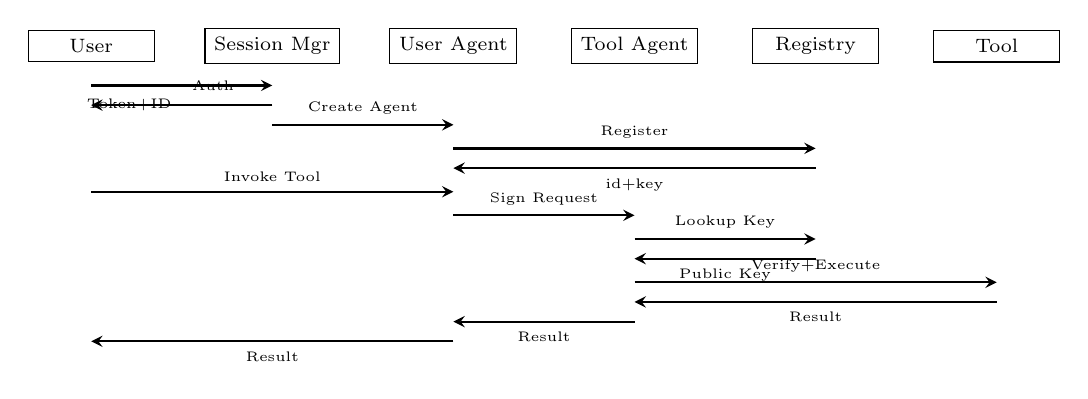
\begin{tikzpicture}[
  node distance=0.2cm,
  entity/.style={rectangle, draw, minimum width=1.6cm, minimum height=0.4cm, font=\scriptsize, align=center},
  arrow/.style={->, thick, >=stealth},
  label/.style={font=\tiny}
]

% Entities at top
\node[entity] (user) at (0,0) {User};
\node[entity] (session) at (2.3,0) {Session Mgr};
\node[entity] (useragent) at (4.6,0) {User Agent};
\node[entity] (toolagent) at (6.9,0) {Tool Agent};
\node[entity] (registry) at (9.2,0) {Registry};
\node[entity] (tool) at (11.5,0) {Tool};

% Authentication phase
\draw[arrow] (0,-0.5) -- node[label, right] {Auth} (2.3,-0.5);
\draw[arrow] (2.3,-0.75) -- node[label, left] {Token+ID} (0,-0.75);

% Agent creation
\draw[arrow] (2.3,-1.0) -- node[label, above] {Create Agent} (4.6,-1.0);

% Registration
\draw[arrow] (4.6,-1.3) -- node[label, above] {Register} (9.2,-1.3);
\draw[arrow] (9.2,-1.55) -- node[label, below] {id+key} (4.6,-1.55);

% Invocation
\draw[arrow] (0,-1.85) -- node[label, above] {Invoke Tool} (4.6,-1.85);
\draw[arrow] (4.6,-2.15) -- node[label, above] {Sign Request} (6.9,-2.15);
\draw[arrow] (6.9,-2.45) -- node[label, above] {Lookup Key} (9.2,-2.45);
\draw[arrow] (9.2,-2.7) -- node[label, below] {Public Key} (6.9,-2.7);

% Verification and execution
\draw[arrow] (6.9,-3.0) -- node[label, above] {Verify+Execute} (11.5,-3.0);
\draw[arrow] (11.5,-3.25) -- node[label, below] {Result} (6.9,-3.25);
\draw[arrow] (6.9,-3.5) -- node[label, below] {Result} (4.6,-3.5);
\draw[arrow] (4.6,-3.75) -- node[label, below] {Result} (0,-3.75);

\end{tikzpicture}
\caption{注册与调用流程：展示认证、实体注册、签名调用及双向验证。}
\label{fig:registration-invocation}
\end{figure*}

本节介绍认证工作流（authenticated workflows）——一种协议级机制，在每次智能体边界穿越时实现确定性验证。
面对具备 A1-A5 能力的攻击者（第~\ref{sec:threat-model}~节），认证工作流提供四项\textbf{密码学保证}，共同实现安全目标 O1-O5：

\textbf{真实性（Authenticity）}（实现 O1：完整性）：每次被接受的调用都通过密码学方式绑定到发起调用的主体（principal）和所执行的操作。攻击者无法在未持有主体私钥的情况下伪造调用，同时绑定 WHO（主体）和 WHAT（操作）。

\textbf{策略绑定（Policy Binding）}（实现 O2-O3：策略执行、权限不可升级）：控制操作的策略通过密码学方式绑定到调用，攻击者无法替换策略而不导致签名失效。

\textbf{篡改证据（Tamper Evidence）}（实现 O4：上下文完整性）：对调用、上下文状态或策略绑定的任何修改，均可通过哈希链和序列号进行密码学检测。

\textbf{不可否认性（Non-Repudiation）}（实现 O5：可问责性）：数字签名创建不可否认的证明，将主体与其操作关联起来，支持带有防篡改审计日志的取证分析和合规验证。

与认证系统调用 \cite{rajagopalan2006,erlingsson2004} 类似，核心思想在概念上很简单：为每次实体间调用附加策略和密码学签名，确保完整性。
{\small
\begin{verbatim}
Invocation = (Args, Policy, MAC)
MAC = Sign(K, Args || Policy)
\end{verbatim}
}
其中，消息认证码（MAC，Message Authentication Code）签名使用密钥或私钥 $K$ 将参数和策略标识符进行密码学绑定。在接收端，验证分三步进行：验证签名以确保真实性和完整性，检索并验证策略绑定以防止替换，然后评估操作是否满足策略规则。

\subsection{设计原则}

实现认证工作流需要四项原则，这些原则组合起来提供密码学保证：

\textbf{零信任身份（Zero-Trust Identity）}：每个实体——智能体、工具、数据源、LLM——拥有唯一的密码学身份（密钥对，keypair）。即使同一进程中的实体也彼此独立验证，不传播任何隐式信任。我们将企业身份与智能体级验证桥接：外部主体通过企业 IAM（身份与访问管理）认证；运行时将这些身份传播为防篡改的会话上下文。内部使用轻量级临时签名标识智能体，应对动态身份挑战（第~\ref{sec:policy}~节）。

\textbf{边界验证（Boundary Verification）}：每次实体间通信——prompt→LLM、agent→tool、tool→data——都需要独立的密码学验证。操作携带签名和策略标识符；接收方使用注册的公钥验证签名，检索策略并评估约束。验证与传输协议无关——在 MCP、LangChain、OpenAI API 或自定义协议中保持一致。

\textbf{策略执行点（Policy Enforcement Points，PEP）}：PEP 在每个边界提供独立验证——实体不能验证自己的操作。PEP 以进程内（链接库）或边车（sidecar）方式部署，在操作执行前验证调用，提供水平可扩展性、零信任验证、防篡改能力和执行独立性。这依赖于 L3（执行完整性）。

\textbf{可信认证上下文（Trustworthy Authenticated Context）}：运行时提供防篡改的会话状态（如 \cite{rajagopalan2025prompts}），确保完整性，包括：将操作绑定到会话范围（上下文 ID、会话 ID）、防重放（序列号）、篡改检测（哈希链，hash chain）以及工作流依赖（证明前置操作已完成的密码学证言）。



\noindent\textbf{协议。}
这些原则组合成一个四阶段协议，每次边界穿越都是一次认证工作流。图~\ref{fig:registration-invocation} 展示了完整流程。

\textbf{注册（Registration）}：每个实体注册后获得 (agent\_id, keypair)。注册在最细粒度进行——智能体内的单个工具获得独立的 (tool\_id, keypair)，最小化爆炸半径（blast radius）。

\textbf{调用（Invocation）}：调用方构造签名调用，绑定操作、参数、策略和会话上下文。

\textbf{验证（Verification）}：接收方 PEP 通过三个阶段独立验证：(1) 签名验证（真实性 + 完整性），(2) 策略绑定验证（防止替换），(3) 策略评估（资源权限、参数约束、证言）。图~\ref{fig:verification-flow} 详细展示了验证流程。

\textbf{证言（Attestation）}：操作完成后，服务对结果签名。上下文用密码学签名的证言更新，证明操作已完成，为下游操作维护认证上下文。


服务对结果签名；调用方在接受结果前验证服务签名——实现类似于双向 TLS 的双向认证（bidirectional authentication）。该无状态协议确保每一步独立验证，无隐式信任在多个工作流步骤中传播。



\begin{figure}[t]
\centering
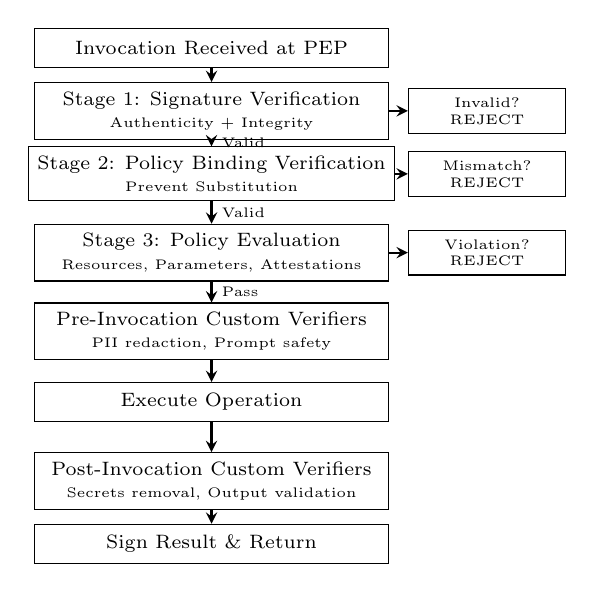
\begin{tikzpicture}[
  node distance=0.4cm,
  box/.style={rectangle, draw, minimum width=4.5cm, minimum height=0.5cm, font=\scriptsize, align=center},
  decision/.style={rectangle, draw, minimum width=2cm, minimum height=0.45cm, font=\tiny, align=center},
  arrow/.style={->, thick, >=stealth}
]

\node[box] (receive) at (0,0) {Invocation Received at PEP};

\node[box] (stage1) at (0,-0.8) {Stage 1: Signature Verification\\{\tiny Authenticity + Integrity}};
\node[decision] (reject1) at (3.5,-0.8) {Invalid?\\REJECT};

\node[box] (stage2) at (0,-1.6) {Stage 2: Policy Binding Verification\\{\tiny Prevent Substitution}};
\node[decision] (reject2) at (3.5,-1.6) {Mismatch?\\REJECT};

\node[box, minimum height=0.7cm] (stage3) at (0,-2.6) {Stage 3: Policy Evaluation\\{\tiny Resources, Parameters, Attestations}};
\node[decision] (reject3) at (3.5,-2.6) {Violation?\\REJECT};

\node[box, minimum height=0.7cm] (pre) at (0,-3.6) {Pre-Invocation Custom Verifiers\\{\tiny PII redaction, Prompt safety}};

\node[box] (execute) at (0,-4.5) {Execute Operation};

\node[box, minimum height=0.7cm] (post) at (0,-5.5) {Post-Invocation Custom Verifiers\\{\tiny Secrets removal, Output validation}};

\node[box] (sign) at (0,-6.3) {Sign Result \& Return};

% Main flow arrows
\draw[arrow] (receive) -- (stage1);
\draw[arrow] (stage1) -- node[right, font=\tiny] {Valid} (stage2);
\draw[arrow] (stage2) -- node[right, font=\tiny] {Valid} (stage3);
\draw[arrow] (stage3) -- node[right, font=\tiny] {Pass} (pre);
\draw[arrow] (pre) -- (execute);
\draw[arrow] (execute) -- (post);
\draw[arrow] (post) -- (sign);

% Reject arrows
\draw[arrow] (stage1.east) -- (reject1.west);
\draw[arrow] (stage2.east) -- (reject2.west);
\draw[arrow] (stage3.east) -- (reject3.west);

\end{tikzpicture}
\caption{PEP 验证流程：三阶段密码学验证及可选的自定义验证器（custom verifier）。}
\label{fig:verification-flow}
\end{figure}
\subsection{验证流程}

图~\ref{fig:verification-flow} 展示了验证流水线——我们完整性主张的核心。该流水线始终强制执行且不可绕过：每次调用在执行前必须经过密码学验证，接收方使用从注册中心检索的公钥独立验证调用方。

\textbf{策略构建}：阶段 3 在接收方通过双视角（dual-perspective）执行独立构建生效策略。PEP 检索组织策略（公司、业务单元、团队）和资源特定约束，计算 $P_{\text{eff}} = \text{Intent} \cap \text{Resource}$（第~\ref{sec:policy}~节）。调用方声明意图由资源约束独立验证——调用方无法影响策略评估。交集代数（定理 1-3）保证单调约束（monotonic restriction）：组合策略只会收窄权限，绝不会放宽。

\textbf{自定义验证器（Custom Verifiers）}：MAPL 的声明式约束处理资源权限和参数，但某些安全检查需要对调用上下文执行命令式逻辑。自定义验证器扩展策略评估，包括 PII（个人身份信息）检测、SQL 注入防护、通过 LLM 分类器（LLMs as judges）的提示安全、速率限制和地理位置检查。调用前（pre-invocation）验证器在策略评估后执行；调用后（post-invocation）验证器处理结果。验证器在密码学验证过的上下文上运行，是由系统管理员（而非应用开发者）检入的受信代码。一旦在验证流程中声明，PEP 强制执行其运行——不可绕过。这在保持完整性保证的同时，提供了特定领域的可扩展性（HIPAA、GDPR、SOC 2）。

四个生产级验证器展示了该架构：(1) MemoryIntegrityVerifier 通过速率限制、受保护字段强制和密码学完整性检查防止内存投毒（OWASP LLM01）；(2) WorkflowIntegrityVerifier 通过强制前置步骤和维护证言链防止工作流劫持（OWASP LLM04）；(3) ToolAuthorizationVerifier 通过 RBAC（基于角色的访问控制）和危险模式检测（如 file\_write→command\_execute）防止工具滥用（OWASP LLM06）；(4) StorageIntegrityVerifier 通过路径遍历防护和加密强制防止数据泄露（OWASP LLM02）。附录~\ref{appendix:verifiers} 提供了实现细节。

这种分离至关重要：核心验证流水线（阶段 1-3：签名验证、策略绑定、策略评估）提供确定性保证——通过 MAPL 声明式约束的密码学强制实现 100\% 召回率且零误报（引理 1、4）。自定义验证器（阶段 4-5）是可选的行政管理扩展，可能使用启发式方法（基于 ML 的 PII 检测、LLM 安全分类器），如果配置不当可能引入误报，但不会削弱核心保证——它们只能增加限制，永不能移除。验证器仅在密码学验证通过后执行，操作对象是经认证的调用和防篡改状态，而非无界应用输入。即使验证器失败或被攻破，阶段 1-3 仍强制执行密码学完整性和策略约束。绕过验证器需要破坏受信管理员代码（L3），而非操纵应用逻辑（A1）。

% Table commented out to save space - examples are inline above
% \begin{table}[h]
% \centering
% \caption{Pluggable verifiers for domain-specific compliance}
% \label{tab:verifiers}
% \scriptsize
% \begin{tabular}{@{}p{2.2cm}p{3cm}p{2.2cm}@{}}
% \toprule
% \textbf{Verifier} & \textbf{Function} & \textbf{Compliance} \\
% \midrule
% PII Detection & Redact sensitive fields & HIPAA, GDPR \\
% SQL Guard & Validate queries & OWASP Top 10 \\
% Rate Limiter & Track invocations & DoS prevention \\
% Cmd Injection & Validate parameters & CWE-78 \\
% Context Check & Verify hash chains & SOC 2, ISO 27001 \\
% Geo Residency & Check location & GDPR Art. 44 \\
% \bottomrule
% \end{tabular}
% \end{table}

\noindent\textbf{安全保证。}面对攻击者 A1-A5（第~\ref{sec:threat-model}~节），协议机制通过四个独立的密码学层次组合成纵深防御：\textbf{完整性}（签名建立真实性，抵御网络攻击 A4）；\textbf{授权}（策略交集强制执行意图——即使持有有效签名，操作也必须满足组合策略，防止应用控制 A1 下的权限升级）；\textbf{溯源}（哈希链和序列号使上下文篡改可检测，抵御内容注入 A2 和多轮操纵 A5）；\textbf{合规}（自定义验证器在密码学验证过的上下文上添加领域特定验证，提供不可否认性）。这些共同实现安全目标 O1-O5。

协议提供纵深防御：每层在每个边界独立运作（引理 7，第~\ref{sec:formal-analysis}~节）。攻破签名验证不会绕过策略评估；篡改上下文不会击败工具 PEP；绕过某个验证器不会使密码学检查失效。第~\ref{sec:formal-analysis}~节形式化了这些独立性保证。
